% !TeX program = pdflatex
%==============================================================================
%  Aula 09 --- Máquinas de Vetores de Suporte (SVM)
%  VERSÃO DO ALUNO: texto para leitura autônoma, fora da sala.
%  (O roteiro de sala é "10 SVM.tex".)
%==============================================================================
\documentclass[11pt,a4paper]{article}
\usepackage[aluno]{../../recursos/latex/estilo-notas}

\title{}
\date{}

\begin{document}
\cabecalhoaula{09}{Máquinas de Vetores de Suporte (SVM)}{AME §8.2 e §4.6; ISLP cap.~9}

%==============================================================================
\section*{O que você vai aprender}
%==============================================================================
Ao final desta aula você deve ser capaz de:
\begin{itemize}[leftmargin=1.4cm]
  \item definir hiperplano separador e o \textbf{classificador de margem máxima};
  \item identificar os \textbf{vetores de suporte} e o papel da margem;
  \item generalizar para dados não separáveis com o \textbf{classificador de vetor
        de suporte} (\emph{soft margin}) e o hiperparâmetro $C$;
  \item explicar o \textbf{truque do \emph{kernel}} a partir da forma dual;
  \item usar \emph{kernels} (polinomial, gaussiano/RBF) para fronteiras não
        lineares e entender $\gamma$;
  \item reconhecer a SVM como minimização da \emph{perda \emph{hinge}} regularizada
        e sua relação com a regressão logística; tratar o caso multiclasse.
\end{itemize}

\noindent
Mudança de perspectiva em relação à Aula~07. Lá, todo método passava por modelar
$\Prob(Y\mid\x)$ e depois aplicar o Teorema de Bayes. A SVM ignora probabilidades e
ataca a fronteira \emph{geometricamente}, procurando a separação mais folgada
possível. É um dos métodos mais elegantes do curso --- liga geometria, otimização e
os RKHS da Aula~04. Comece pela pergunta:

\begin{center}\itshape
  se há infinitos hiperplanos que separam as classes, qual é o melhor?
\end{center}

%==============================================================================
\section{Hiperplanos e o classificador de margem máxima}
%==============================================================================
Codifique as classes como $y\in\{-1,+1\}$. Um \textbf{hiperplano} em $\R^p$ é o
conjunto $\{\x: f(\x)=0\}$ com $f(\x)=\beta_0+\bbeta^\top\x$. Ele separa o espaço
em dois lados conforme o sinal de $f$. Dizemos que os dados são \emph{linearmente
separáveis} se existe $f$ tal que
\begin{equation}\label{eq:sep}
  y_i\,f(\X_i) > 0 \qquad \text{para todo } i.
\end{equation}
A magnitude $\abs{f(\x)}$ (com $\norm{\bbeta}=1$) é a \emph{distância} de $\x$ ao
hiperplano.

\begin{ideia}[por que a codificação $\pm1$]
Não é capricho de notação. Com $y\in\{-1,+1\}$, o produto $y_i f(\X_i)$ é positivo
exatamente quando a classificação está certa, e seu \emph{valor} mede o quanto ela
está certa. Essa única quantidade --- a \textbf{margem} da observação $i$ --- vai
organizar a aula inteira, inclusive a função de perda da
Seção~\ref{sec:hinge}.
\end{ideia}

\begin{definicao}[Classificador de margem máxima]
Procura-se o hiperplano que maximiza a margem $M$:
\[
  \max_{\beta_0,\bbeta}\ M \quad\text{s.a.}\quad
  \sum_{j=1}^p \beta_j^2 = 1,\qquad
  y_i\,f(\X_i)\ge M \ \ \forall i.
\]
A restrição $\norm{\bbeta}=1$ torna os hiperplanos comparáveis (assim $y_if(\X_i)$
é a distância com sinal). As observações que \emph{atingem} a margem
($y_if(\X_i)=M$) são os \textbf{vetores de suporte}.
\end{definicao}

\begin{atencao}
Apenas os vetores de suporte determinam o hiperplano: mover um ponto longe da
margem não muda \emph{nada}. Isso é bom e ruim ao mesmo tempo. Bom: o modelo é
econômico, definido por um punhado de observações. Ruim: a formulação \emph{exige}
separabilidade perfeita e é \textbf{muito sensível} --- mover um único vetor de
suporte pode girar a fronteira inteira. Precisamos relaxá-la.
\end{atencao}

%==============================================================================
\section{O classificador de vetor de suporte (\emph{soft margin})}
%==============================================================================
Para lidar com dados não separáveis (e ganhar robustez), permitimos que algumas
observações violem a margem, introduzindo \emph{folgas} $e_i\ge 0$:
\begin{equation}\label{eq:soft}
  \max_{\beta_0,\bbeta,\,\bm{e}}\ M \quad\text{s.a.}\quad
  \norm{\bbeta}=1,\quad
  y_i\,f(\X_i)\ge M(1-e_i)\ \ \forall i,\quad
  e_i\ge 0,\ \ \sum_{i=1}^n e_i \le C.
\end{equation}
A folga $e_i$ mede o quanto a $i$-ésima observação viola a margem: $e_i>0$ significa
dentro da margem; $e_i>1$ significa do \emph{lado errado} do hiperplano (erro de
classificação).

\begin{figure}[htbp]
  \centering
  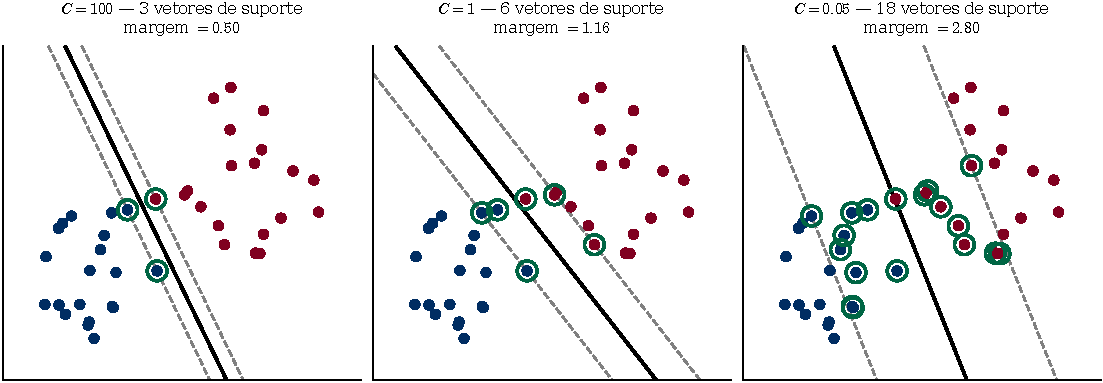
\includegraphics[width=\textwidth]{../../recursos/figuras/09-margem.pdf}
  \caption{O mesmo conjunto de $40$ pontos com três orçamentos de violação. A linha
  cheia é a fronteira; as tracejadas delimitam a margem; os pontos circulados em
  verde são os \textbf{vetores de suporte}. Aumentar a tolerância a violações alarga
  a margem e traz mais pontos para dentro dela: de $3$ vetores de suporte e margem
  $0{,}50$ até $18$ vetores de suporte e margem $2{,}80$. Quanto mais pontos
  sustentam a solução, menos ela depende de cada um --- daí a robustez.
  \textbf{Atenção ao rótulo:} este é o \texttt{C} do \texttt{scikit-learn}, cuja
  convenção é a inversa da de \eqref{eq:soft}.}
  \label{fig:margem}
\end{figure}

\begin{ideia}
$C$ é o \textbf{tuning parameter}, escolhido por validação cruzada (Aula~03). Na
convenção de \eqref{eq:soft} --- a do [AME] e do [ISLP] --- $C$ é o \emph{orçamento
de violações}:
\begin{itemize}[leftmargin=1.2cm,nosep]
  \item $C$ \emph{grande}: tolera muitas violações $\Rightarrow$ margem larga, mais
        vetores de suporte, modelo mais \emph{rígido} (alto viés, baixa variância);
  \item $C$ \emph{pequeno}: poucas violações $\Rightarrow$ margem estreita, modelo
        mais \emph{flexível} (baixo viés, alta variância).
\end{itemize}
É o balanço viés--variância da Aula~01 outra vez.
\end{ideia}

\begin{atencao}[a inversão que já derrubou muita gente]
No \texttt{scikit-learn}, o \texttt{C} é o \emph{peso da penalidade} sobre as
violações, não o orçamento delas. Portanto tudo se inverte: \texttt{C} grande
penaliza mais, tolera menos, e dá margem \emph{estreita}. É o que a
Figura~\ref{fig:margem} mostra. Ao ler qualquer texto sobre SVM, confira qual
convenção está em uso antes de interpretar ``$C$ grande''.
\end{atencao}

%==============================================================================
\section{O truque do \emph{kernel}}
%==============================================================================
A chave que torna a SVM poderosa: a solução depende dos dados \emph{apenas através
de produtos internos}. Pode-se mostrar que a função ótima se escreve
\begin{equation}\label{eq:dual}
  f(\x) = \beta_0 + \sum_{k=1}^n \alpha_k\,\inner{\x}{\X_k},
  \qquad \inner{\x}{\X_k}=\textstyle\sum_{j=1}^p x_j x_{k,j},
\end{equation}
e que o cálculo dos $\alpha_k$ também só requer os produtos internos
$\inner{\X_i}{\X_k}$ entre as observações. Crucialmente, $\alpha_k=0$ para todos os
pontos que \emph{não} são vetores de suporte; logo
\[
  f(\x) = \beta_0 + \sum_{k\in S}\alpha_k\,\inner{\x}{\X_k},
\]
onde $S$ é o conjunto de vetores de suporte.

\begin{ideia}
Como tudo depende só de produtos internos, podemos \textbf{substituir}
$\inner{\x}{\X_k}$ por um \emph{kernel} $K(\x,\X_k)$ --- que corresponde a um produto
interno num espaço de \emph{features} de dimensão muito maior (ou infinita), sem
\emph{nunca} computar esse espaço explicitamente. Isso é o \textbf{truque do
\emph{kernel}}: fronteiras não lineares no espaço original a custo de fronteiras
lineares num espaço ampliado.
\end{ideia}

\begin{exemplo}[o truque em duas dimensões]
Tome $K(\x,\x')=(\inner{\x}{\x'})^2$ em $\R^2$. Expandindo,
\[
  (x_1x_1'+x_2x_2')^2 = (x_1^2)(x_1'^2) + 2(x_1x_2)(x_1'x_2') + (x_2^2)(x_2'^2)
  = \inner{\phi(\x)}{\phi(\x')},
\]
com $\phi(\x)=(x_1^2,\;\sqrt2\,x_1x_2,\;x_2^2)$. Ou seja: calcular \emph{um} produto
e elevá-lo ao quadrado equivale a mapear os pontos para $\R^3$ e fazer o produto
interno lá. Com o kernel polinomial de grau $p$ em $\R^p$ o espaço tem dimensão
$\binom{p+p}{p}$, e com o RBF ele é \emph{de dimensão infinita} --- e o custo
continua sendo uma conta com $p$ termos. É esse o negócio.
\end{exemplo}

\noindent \emph{Kernels} de Mercer comuns (cf.\ Aula~04, §4.6):
\begin{center}\small
\renewcommand{\arraystretch}{1.4}
\begin{tabular}{@{}ll@{}}
\toprule
\textbf{Kernel} & \textbf{$K(\x,\x')$} \\
\midrule
Linear      & $\inner{\x}{\x'}$ \\
Polinomial  & $(1+\inner{\x}{\x'})^{p}$ \\
Gaussiano (RBF) & $\exp\!\big(-\gamma\,\norm{\x-\x'}^2\big)$ \\
\bottomrule
\end{tabular}
\end{center}
No kernel gaussiano, $\gamma>0$ é um \emph{tuning parameter}: $\gamma$ grande
$\Rightarrow$ influência local, fronteiras muito flexíveis (risco de superajuste);
$\gamma$ pequeno $\Rightarrow$ fronteiras suaves. Escolhem-se $C$ e $\gamma$ juntos
por validação cruzada.

\begin{figure}[htbp]
  \centering
  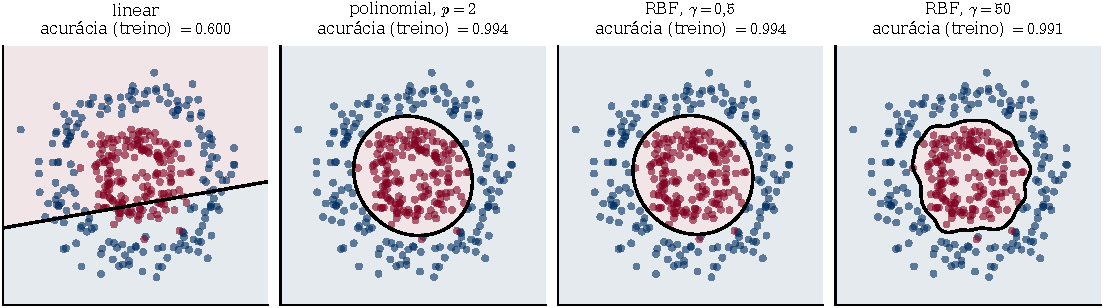
\includegraphics[width=\textwidth]{../../recursos/figuras/09-kernel.pdf}
  \caption{Duas classes dispostas em anéis concêntricos --- o exemplo canônico do
  que uma reta não resolve. O kernel linear acerta $60\%$, pouco acima do palpite. O
  polinomial de grau~2 encontra a circunferência exata e sobe para $99{,}4\%$, e o
  RBF com $\gamma=0{,}5$ faz o mesmo. Já o RBF com $\gamma=50$ produz uma fronteira
  rendilhada que persegue observações individuais: $\gamma$ é um botão de
  flexibilidade e, como todos os outros do curso, superajusta se você o girar demais.}
  \label{fig:kernel}
\end{figure}

%==============================================================================
\section{SVM como perda \emph{hinge} regularizada}\label{sec:hinge}
%==============================================================================
Há uma leitura que conecta a SVM a tudo o que vimos. Dado um kernel de Mercer $K$
com RKHS $\mathcal{H}_K$ (Aula~04), o classificador da SVM minimiza
\begin{equation}\label{eq:hinge}
  \min_{g\in\mathcal{H}_K}\ \sum_{k=1}^n \underbrace{\big(1-y_k\,g(\X_k)\big)_+}_{\text{perda \emph{hinge}}}
  + \lambda\,\norm{g}_{\mathcal{H}_K}^2 ,
\end{equation}
onde $(u)_+=\max(u,0)$. Ou seja, a SVM é \emph{ajuste de perda + regularização}
(Aula~02), com a \textbf{perda \emph{hinge}} $L(y,g)=(1-yg)_+$.

\begin{observacao}
A perda \emph{hinge} é \textbf{zero} quando $y\,g(\x)\ge 1$, isto é, quando o ponto
está do lado certo e \emph{folgadamente} longe da margem. Só os pontos próximos ou
violando a margem contribuem --- e são exatamente os \emph{vetores de suporte}. No
caso separável, \eqref{eq:hinge} reencontra a margem máxima ($1/\norm{g}$).
\end{observacao}

\begin{figure}[htbp]
  \centering
  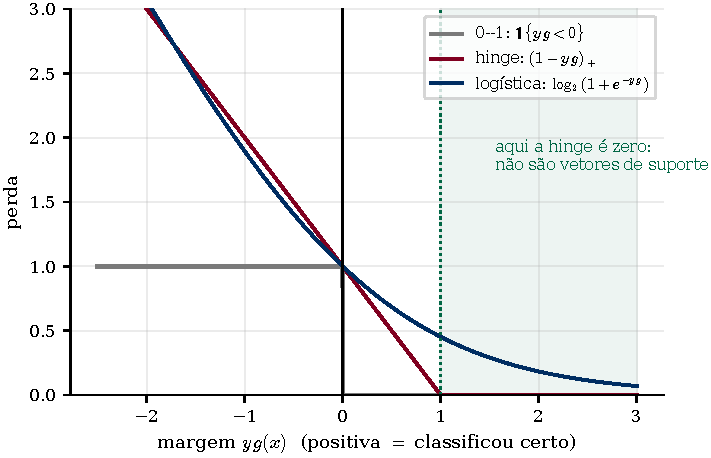
\includegraphics[width=0.62\textwidth]{../../recursos/figuras/09-perdas.pdf}
  \caption{As três perdas como função da margem $y\,g(x)$. A 0--1 é o que
  gostaríamos de minimizar, mas ela é descontínua e constante por partes --- otimizar
  sobre ela é NP-difícil. A \emph{hinge} e a logística são substitutas convexas:
  ambas majoram a 0--1 e são tratáveis. A diferença decisiva está na faixa
  sombreada: a \emph{hinge} \textbf{zera} a partir da margem $1$, e todos os pontos
  ali param de influenciar a solução --- é daí que vem a esparsidade em vetores de
  suporte. A logística nunca chega a zero, e por isso \emph{todo} ponto pesa um
  pouco.}
  \label{fig:perdas}
\end{figure}

\subsection{Relação com a regressão logística}
A SVM (\emph{hinge}) e a regressão logística (perda logística
$\log(1+e^{-yg})$) são ambas ``perda de margem $+$ regularização $\ell_2$'':
\begin{itemize}[leftmargin=1.4cm,nosep]
  \item a \emph{hinge} é exatamente zero longe da margem $\Rightarrow$ solução
        \emph{esparsa} em vetores de suporte; a logística nunca é zero;
  \item a logística entrega \textbf{probabilidades} calibradas (Aula~08); a SVM
        entrega só a fronteira. As ``probabilidades'' do \texttt{SVC} vêm de um
        ajuste \emph{a posteriori} (escala de Platt), não do método.
\end{itemize}
Regra prática: classes bem separadas $\to$ SVM costuma ir muito bem; quando se quer
$\Prob(Y\mid\x)$, prefira a logística.

%==============================================================================
\section{Mais de duas classes}
%==============================================================================
A SVM é intrinsecamente binária --- não há como escrever ``$y_i f(\X_i)>0$'' com
três classes. Para $\abs{\mathcal{C}}>2$, contorna-se com vários classificadores
binários:
\begin{description}[leftmargin=2.8cm,style=nextline]
  \item[Um-contra-um (OvO)] treina uma SVM para cada par de classes
        ($\binom{K}{2}$ classificadores) e classifica por votação. Cada ajuste usa
        só os dados de duas classes, então são muitos problemas pequenos. Padrão do
        \texttt{scikit-learn}.
  \item[Um-contra-todos (OvA)] treina $K$ SVMs (cada classe vs.\ o resto) e escolhe
        a de maior $f(\x)$. São $K$ problemas grandes, e cada um deles fica
        desbalanceado --- com a ressalva da Aula~08.
\end{description}

%==============================================================================
\section{Prática em Python}
%==============================================================================
\begin{lstlisting}
from sklearn.svm import SVC
from sklearn.preprocessing import StandardScaler
from sklearn.pipeline import make_pipeline
from sklearn.model_selection import GridSearchCV

# SVM com kernel RBF; padronizar e ESSENCIAL (metodo baseado em distancia)
pipe = make_pipeline(StandardScaler(), SVC(kernel="rbf"))
grade = {"svc__C":     [0.1, 1, 10, 100],
         "svc__gamma": [0.001, 0.01, 0.1, 1]}
busca = GridSearchCV(pipe, grade, cv=5, scoring="accuracy")
busca.fit(X_tr, y_tr)
print("melhores parametros:", busca.best_params_)

# Para probabilidades: SVC(probability=True) (usa Platt scaling, mais lento)
\end{lstlisting}

\begin{atencao}
Três observações práticas. (i) SVM com RBF é \textbf{sensível à escala} --- a
distância $\norm{\x-\x'}^2$ do kernel soma todas as coordenadas, então
\emph{sempre} padronize dentro do \emph{pipeline} (Aula~06). (ii) $C$ e $\gamma$
interagem, e por isso a busca é numa \emph{grade bidimensional}, não em dois passos
separados. (iii) O custo de treino do \texttt{SVC} cresce entre $O(n^2)$ e
$O(n^3)$: com centenas de milhares de observações ele fica inviável, e a saída é o
\texttt{LinearSVC} ou aproximações de kernel (\texttt{Nystroem}).
\end{atencao}

Os notebooks \texttt{Aula prática 09} e \texttt{Exemplo - SVM em dados artificiais}
ilustram o efeito de $C$,
$\gamma$ e da escolha do kernel sobre a fronteira de decisão.

%==============================================================================
\section*{Resumo}
%==============================================================================
\begin{itemize}[leftmargin=1.4cm]
  \item \textbf{Margem máxima}: hiperplano separador de maior folga; definido pelos
        \emph{vetores de suporte}; exige separabilidade e é frágil.
  \item \textbf{\emph{Soft margin}} \eqref{eq:soft}: folgas $e_i$ e orçamento $C$
        controlam o balanço viés--variância (Fig.~\ref{fig:margem}). Cuidado com a
        convenção invertida de $C$ no \texttt{scikit-learn}.
  \item \textbf{Truque do kernel}: a solução só depende de produtos internos
        \eqref{eq:dual}; trocá-los por $K$ dá fronteiras não lineares
        (Fig.~\ref{fig:kernel}), e $\gamma$ do RBF é mais um botão de flexibilidade.
  \item SVM $=$ \textbf{perda \emph{hinge}} $+$ regularização \eqref{eq:hinge}
        (RKHS, Aula~04); a hinge zera longe da margem, e é daí que vem a esparsidade
        (Fig.~\ref{fig:perdas}).
  \item Relação com a logística (perda de margem $+$ $\ell_2$); SVM não dá
        probabilidades de imediato.
  \item Multiclasse por OvO/OvA; \emph{padronize} sempre.
\end{itemize}

\paragraph{Leitura recomendada.} [AME] §8.2 (SVM) e §4.6 (RKHS e o truque do
kernel, onde o mesmo maquinário aparece em regressão). [ISLP] Capítulo~9 inteiro:
§9.1 (margem máxima), §9.2 (vetor de suporte e o papel de $C$ --- a Figura~9.7 deles
é a nossa Figura~\ref{fig:margem}), §9.3 (kernels, com a versão deles da nossa
Figura~\ref{fig:kernel}), §9.4 (multiclasse) e §9.5 (relação com a logística, de
onde vem a nossa Figura~\ref{fig:perdas}).

\paragraph{Para praticar.} \texttt{Lista teorica 09.pdf} (teórica, com gabarito) e \texttt{Lista prática 09.ipynb} (prática, para completar as lacunas), nesta mesma pasta.

\end{document}
